\section{pbdR}

\hidenum
\begin{frame}[noframenumbering]
\frametitle{Contents}
 \tableofcontents[currentsection,hideothersubsections,sectionstyle=show/hide]
\end{frame}
\shownum


\subsection{The pbdR Project}


\begin{frame}
  \begin{block}{Programming with Big Data in R (pbdR)}
       \centering Striving for \emph{Productivity, Portability, Performance}\\[.4cm]\pause
  \begin{columns}[onlytextwidth]
    \begin{column}{0.30\textwidth}
      \centering
       
\includegraphics[width=3.4cm]{pics/simple}\\[.2cm]
    \end{column}
    \begin{column}{0.65\textwidth}
  \begin{itemize}[<+-|alert@+>]
    \item Series of \emph{free}\footnote{MPL, BSD, and GPL licensed} R packages.
    \item Scalable, big data analytics with high-level syntax.
    \item Implicit management of distributed data details.
    \item Methods have syntax \emph{identical} to R.
    \item Powered by state of the art numerical libraries (MPI, ScaLAPACK, PBLAS, BLACS, LAPACK, BLAS, \dots)
  \end{itemize}
    \end{column}
​  \end{columns}
\end{block}
\end{frame}




\begin{frame}[shrink]
  \begin{block}{pbdR Packages}
    \begin{center}
        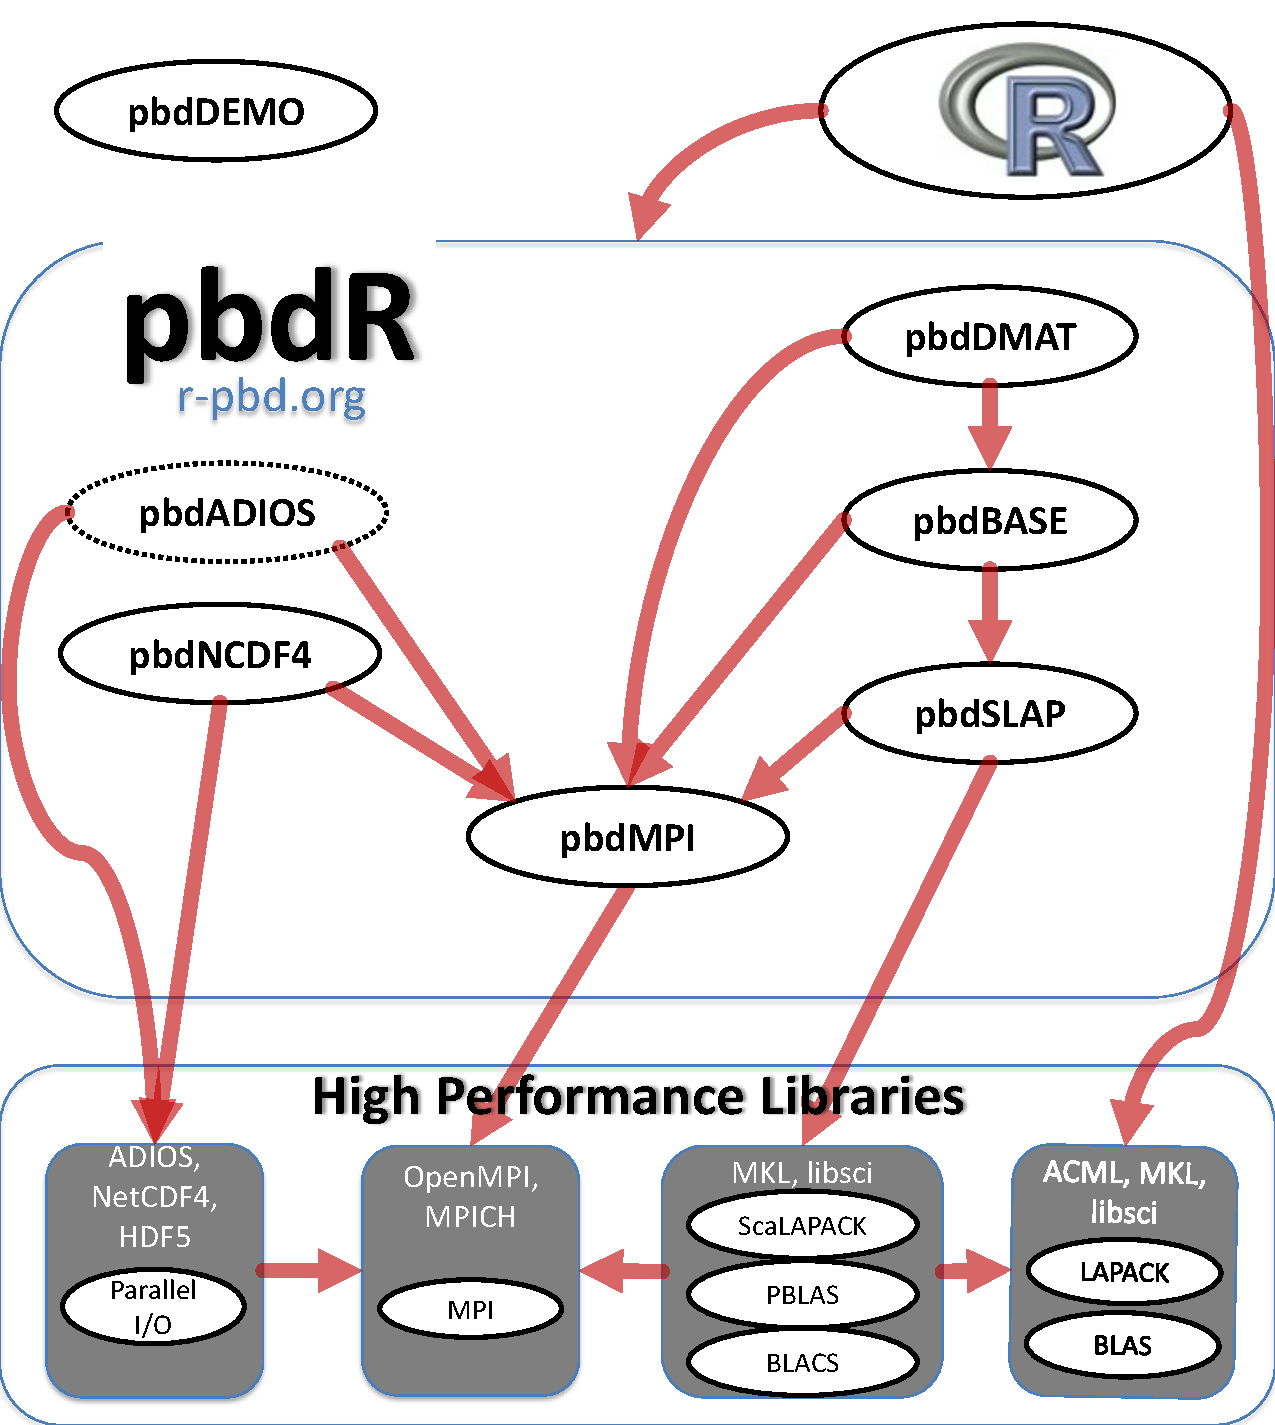
\includegraphics[width=7cm, height=7cm]{pics/pbdpacks}
    \end{center}
  \end{block}
\end{frame}


\begin{frame}[shrink]
  \begin{block}{pbdR Packages --- http://code.r-pbd.org}\pause
  Released to CRAN:
  \begin{itemize}[<+-|alert@+>]
    \item \pkg{pbdMPI}: MPI bindings (explicit, low-level)
    \item \pkg{pbdSLAP}: Foreign library (just install it, nothing to use)
    \item \pkg{pbdBASE}: Compiled code (used by DMAT, also for devs)
    \item \pkg{pbdDMAT}: Distributed matrices (mostly implicit, high-level)
    \item \pkg{pbdNCDF4}: Parallel NetCDF4 reader
    \item \pkg{pbdDEMO}: Package demonstrations, examples, vignette written in textbook style
  \end{itemize}
%     \\[.2cm]
    Future Development:
  \begin{itemize}[<+-|alert@+>]
    \item Profiling tools
    \item Client/server interface for interactive sessions
    \item \dots
  \end{itemize}
  \end{block}
\end{frame}



\begin{frame}[fragile]
  \begin{block}{Example Syntax}\pause
  \begin{lstlisting}
x <- x[-1, 2:5]
x <- log(abs(x) + 1)
xtx <- t(x) %*% x
ans <- svd(solve(xtx))
  \end{lstlisting}
  \begin{center}
  \pause Look familiar?\\[.4cm] \pause
  \emph{The above runs on 1 core with R or 10,000 cores with pbdR}
  \end{center}
  \end{block}
\end{frame}



\subsection{pbdR Paradigms}

%%%%%% FIXME
%% distributed
%% batch
%% spmd
%% OO
%% ...?


\begin{frame}
  \begin{block}{pbdR Focus:  Distributed Machines}
   \begin{center}
    \begin{minipage}[t]{.47\textwidth}
    \begin{block}{\centering Shared Memory Machines}
    \begin{center}
    Thousands of cores\\[.2cm]
    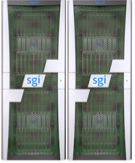
\includegraphics[scale=.65]{pics/nautilus}\\
    {\tiny \emph{Nautilus}, University of Tennessee\\1024 cores}
    \end{center}
    \end{block}
    \end{minipage}
    \hspace{.1cm}
    \begin{minipage}[t]{.47\textwidth}
    \begin{block}{\centering Distributed Memory Machines}
    \begin{center}
    Hundreds of thousands of cores\\[.2cm]
    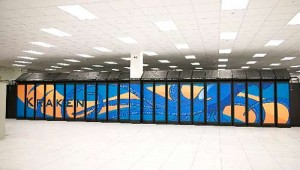
\includegraphics[width=.95\textwidth]{pics/kraken}\\
    {\tiny \emph{Kraken}, University of Tennessee\\ 112,896 cores}
    \end{center}
    \end{block}
    \end{minipage}
    \end{center}
    \end{block}
\end{frame}

\begin{frame}
  \begin{block}{pbdR Paradigms}
  Programs that use pbdR are meant to utilize the:
  \begin{itemize}[<+-|alert@+>]
   \item Data Parallelism method
   \item Single Program/Multiple Data (SPMD) style
  \end{itemize}
  \end{block}
\end{frame}



\begin{frame}
  \begin{block}{SPMD}\pause
  The pbdR Packages enable high-level ``Single Program/Multiple Data'' (SPMD) programming:
    \begin{itemize}
      \item SPMD is a programming \emph{paradigm}.
      \item Arguably the simplest extension of serial programming.
      \item Sort of like trying to explain breathing \dots
      \item Not to be confused with SIMD.
      \item SPMD utilizes MIMD architecture computers.
      \item Only one program is written, executed in batch independently on all processors.
      \item Different processors are autonomous; there is no manager.
%       \item Like ``Map/Reduce'', you probably used it without knowing it even had a name.
    \end{itemize}
  \end{block}
\end{frame}


\begin{frame}[fragile]
  \begin{block}{SPMD}\pause
      SPMD codes are run in batch (non-interactively):
\begin{lstlisting}[backgroundcolor=\color{white},keywordstyle=\color{black},title=From the Shell]
mpirun -np 4 Rscript my_script.R
\end{lstlisting}
  \end{block}
\end{frame}


\begin{frame}
  \begin{block}{pbdR Paradigms:  Data Parallelism}
  With data parallelism:
  \begin{itemize}[<+-|alert@+>]
   \item No one processor/node owns all the data.
   \item Processors own local pieces of a (conceptually) global object
  \end{itemize}
  \end{block}
\end{frame}


\begin{frame}
  \begin{block}{pbdR Paradigms:  SPMD}
  \begin{itemize}[<+-|alert@+>]
   \item Natural extension of writing serial codes.
   \item Different from Manager/Worker.
   \item No one processor is in charge. Each thinks it's the boss (``it's like academia'').
   \item One program written, executed independently by all processors.
   \item Each processor owns a local sub-piece of data from the (conceptual) whole.
  \end{itemize}
  \end{block}
\end{frame}

% 
% \begin{frame}
%   \begin{block}{Manager/Worker vs SPMD}
%    \begin{center}
%    Graphics will go here\\
%     \begin{minipage}[t]{.47\textwidth}
%     \begin{block}{\centering Manager/Worker:  Fascism}
% %image
%     \end{block}
%     \end{minipage}
%     \hspace{.1cm}
%     \begin{minipage}[t]{.47\textwidth}
%     \begin{block}{\centering SPMD: Democracy}
% %image 
%     \end{block}
%     \end{minipage}
%     \end{center}
%     \end{block}
% \end{frame}